\documentclass[a4paper,11pt]{article}
\usepackage{fancyhdr}
\usepackage{fancyheadings}
\usepackage[american]{babel}
\usepackage[utf8]{inputenc}
\usepackage[active]{srcltx}
\usepackage{algorithm}
\usepackage[noend]{algorithmic}
\usepackage{amsmath}
\usepackage{amssymb}
\usepackage{amsthm}
\usepackage{bbm}
\usepackage{enumerate}
\usepackage{graphicx}
\usepackage{ifthen}
\usepackage{listings}
\usepackage{struktex}
\usepackage{hyperref}

\usepackage{braket}

\renewcommand{\vector}[2]{{\left(\begin{array}{c} #1 \\ #2 \end{array}\right)}}

%%%%%%%%%%%%%%%%%%%%%%%%%%%%%%%%%%%%%%%%%%%%%%%%%%%%%%
%%%%%%%%%%%%%% EDIT THIS PART %%%%%%%%%%%%%%%%%%%%%%%%
%%%%%%%%%%%%%%%%%%%%%%%%%%%%%%%%%%%%%%%%%%%%%%%%%%%%%%
\newcommand{\Fach}{Basics of Quantum Information and Computing}
\newcommand{\Name}{Michael Hartmann}
\newcommand{\Lehrstuhl}{Theoretische Physik I, Universität Augsburg}
\newcommand{\Uebungsblatt}{3} %  <-- UPDATE ME
\newcommand{\Date}{25.11.2016} %  <-- UPDATE ME
%%%%%%%%%%%%%%%%%%%%%%%%%%%%%%%%%%%%%%%%%%%%%%%%%%%%%%
%%%%%%%%%%%%%%%%%%%%%%%%%%%%%%%%%%%%%%%%%%%%%%%%%%%%%%

\DeclareMathOperator{\Tr}{Tr}

\setlength{\parindent}{0em}
\topmargin -1.0cm
\oddsidemargin 0cm
\evensidemargin 0cm
\setlength{\textheight}{9.2in}
\setlength{\textwidth}{6.0in}

%%%%%%%%%%%%%%%
%% Problem-COMMAND
\newcommand{\Problem}[1]{
  {
  \vspace*{0.5cm}
  \textsf{\textbf{Problem #1}}
  \vspace*{0.2cm}
  
  }
}
%%%%%%%%%%%%%%
\hypersetup{
    pdftitle={\Fach{}: Exercise \Uebungsblatt{}},
    pdfauthor={\Name},
    pdfborder={0 0 0}
}

\lstset{ %
language=java,
basicstyle=\footnotesize\tt,
showtabs=false,
tabsize=2,
captionpos=b,
breaklines=true,
extendedchars=true,
showstringspaces=false,
flexiblecolumns=true,
}

\title{Exercise \Uebungsblatt{}}
\author{\Name{}}

\begin{document}
\thispagestyle{fancy}
\lhead{\sf \Fach{} \\ \tiny{\Name, \Lehrstuhl}}
\rhead{\sf \Date{}}
\vspace*{0.2cm}
\begin{center}
\LARGE \sf \textbf{Exercise \Uebungsblatt{} -- A Quantum Game}
\end{center}
\vspace*{0.2cm}

%%%%%%%%%%%%%%%%%%%%%%%%%%%%%%%%%%%%%%%%%%%%%%%%%%%%%%
%% Insert your solutions here %%%%%%%%%%%%%%%%%%%%%%%%
%%%%%%%%%%%%%%%%%%%%%%%%%%%%%%%%%%%%%%%%%%%%%%%%%%%%%%

\begin{figure}[h!]
\centering
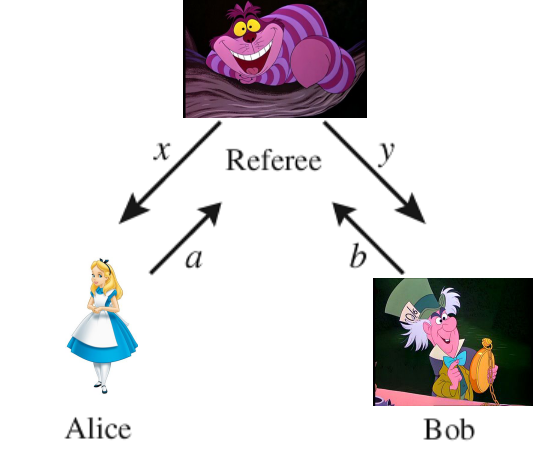
\includegraphics[scale=0.47]{images/alicebob.png}
\caption{The referee distributes the bits $x$ and $y$ to Alice and Bob in the first round. Alice and Bob return the bits $a$ and $b$ to the referee.}
\label{game}
\end{figure}

Alice and Bob play a game. The game begins with a referee selecting two bits
$x$ and $y$ uniformly at random. He then sends $x$ to Alice and $y$ to Bob.
Alice and Bob are not allowed to communicate in any way at this point. Alice
sends back to the referee a bit $a$, and Bob sends back a bit $b$ (see Fig. \ref{game}).
Since they are spatially separated, Alice's bit $a$ can only depend on $x$, and
similarly, Bob's bit $b$ can only depend on $y$. The referee then determines if
the \texttt{AND} of $x$ and $y$ is equal to the \texttt{XOR} of $a$ and $b$. If
so, Alice and Bob win the game. That is, the winning condition is
\begin{equation}
x \wedge y = a \oplus b.
\end{equation}

\begin{enumerate}[a)]
    \item Make a table that presents the winning conditions depending on the
    various different values of $x$, $y$, $a$ and $b$.

    \item Remember that $a=a(x)$ and $b=b(y)$. What is an optimal strategy and
    what is the maximal winning propability?

    \item Let's assume Alice and Bob share a two-qubit system wich is
    initialized in the Bell state
    \begin{equation}
    \ket{\Psi} = \frac{1}{\sqrt 2} \left( \ket{00} + \ket{11}\right).
    \end{equation}
    Alice and Bob agree to use the following strategy:
    \begin{enumerate}[1.]
    \item Alice takes the first qubit and Bob takes the second qubit from the quantum system.
    \item If Alice receives $x=0$, she does not apply any operation on her
    qubit. If Alice receives $x=1$, she applies a rotation by $\pi/4$.
    \item If Bob receives $y=0$, he applies a rotation by $\pi/8$. If Bob receives $y=1$, he applies a rotation by $-\pi/8$.
    \item Alice and Bob meassure their qubits and output the values obtained as
    their answers $a$ and $b$.
    \end{enumerate}

    What is the winning propability?
\end{enumerate}


\end{document}
